% Insert after the report's existing \appendix command.
% Replace overlapping E1 appendix material rather than duplicating it.

\section{Supporting Evidence for E1}
\label{app:e1story}

\subsection{Application Payload Goodput}

Goodput was calculated by summing application payload bytes for
successful completions inside each measurement window, multiplying
by eight and dividing by window duration. JSON metadata and protocol
headers were excluded. Figure~\ref{fig:e1story-goodput} shows the mean
of three run-level goodput measurements with minimum--maximum bars.

\begin{figure}[htbp]
    \centering
    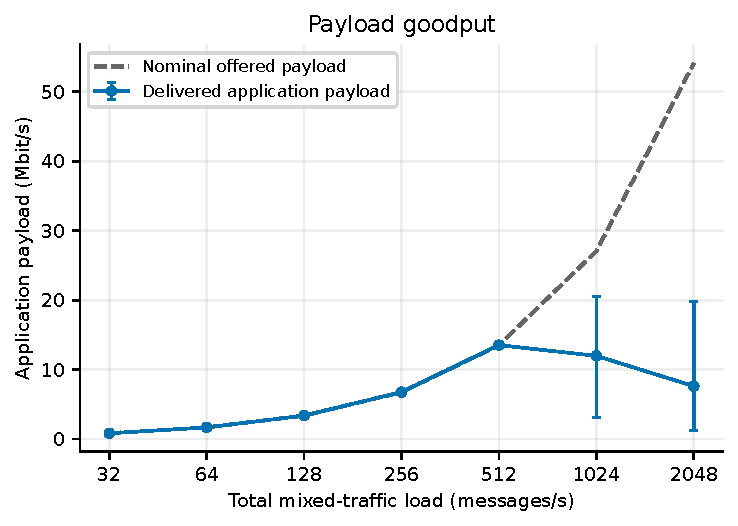
\includegraphics[width=\columnwidth]{figures/appendix_goodput.pdf}
    \caption{Delivered application payload goodput. The dashed line
    shows nominal offered payload rate. Points are means of three runs;
    error bars show minimum--maximum.}
    \label{fig:e1story-goodput}
\end{figure}

At 16 equivalents, delivered payload goodput was approximately
13.53 Mbit/s, matching the nominal offered payload rate. At
64 equivalents, it averaged 7.62 Mbit/s despite a nominal offered
rate of 54.12 Mbit/s. Requests/s and payload Mbit/s are complementary:
message sizes differ, and overflow can change the delivered class mix.

\subsection{FIFO Admission Drops}

For each run, FIFO admission drops among messages generated during
measurement were divided by the total generated-message count.
Figure~\ref{fig:e1story-drops} averages these run-level percentages.
This differs from the pooled-count calculation in
Table~\ref{tab:e1story-summary}, although the high-load values round
to the same displayed percentages.

\begin{figure}[htbp]
    \centering
    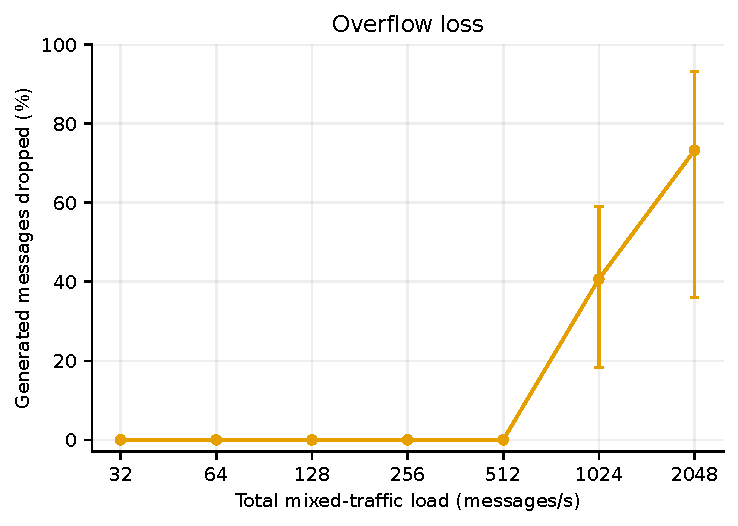
\includegraphics[width=\columnwidth]{figures/appendix_drops.pdf}
    \caption{Generated messages discarded at FIFO admission.
    Points average three run-level percentages; error bars show
    minimum--maximum.}
    \label{fig:e1story-drops}
\end{figure}

No FIFO drops occurred through 16 equivalents. Mean per-run drop
fractions reached 40.68\% at 32 equivalents and 73.27\% at
64 equivalents. These are queue-admission losses: the dropped
messages were never sent as HTTP requests. They are not measurements
of TCP packet loss.

\subsection{Queue Development during Individual Runs}

Queue state was reconstructed from timestamped events and sampled
every 100 ms during repeat 1 at 16, 32 and 64 equivalents.
Figure~\ref{fig:e1story-trace} contains individual traces rather than
averages across repetitions; its curves identify load conditions.

\begin{figure}[htbp]
    \centering
    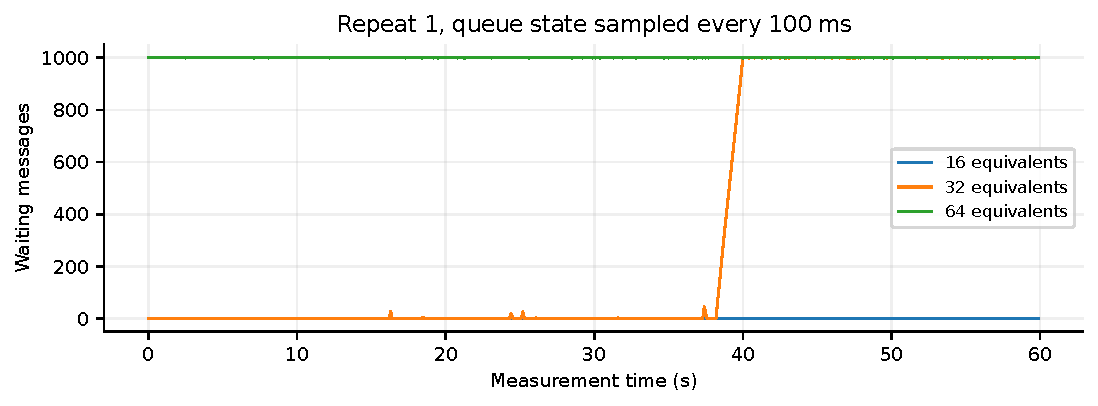
\includegraphics[width=\columnwidth]{figures/appendix_queue_trace.pdf}
    \caption{Waiting-queue occupancy sampled every 100 ms during
    repeat 1 of the three highest load conditions. This fixed selection
    is not presented as representative of every repetition.}
    \label{fig:e1story-trace}
\end{figure}

The traces show when backlog develops within a run, which a whole-run
average cannot reveal. Conclusions across repetitions should be based
on the load-sweep statistics rather than these selected traces alone.

\subsection{Variation within the 32-Equivalent, Repeat-1 Run}

This run was divided into consecutive 10-second bins. Cumulative CPU
counters were interpolated at each boundary, and CPU-time increments
were divided by bin duration. Figure~\ref{fig:e1story-within-cpu}
connects bin averages, rather than instantaneous CPU samples.

\begin{figure}[htbp]
    \centering
    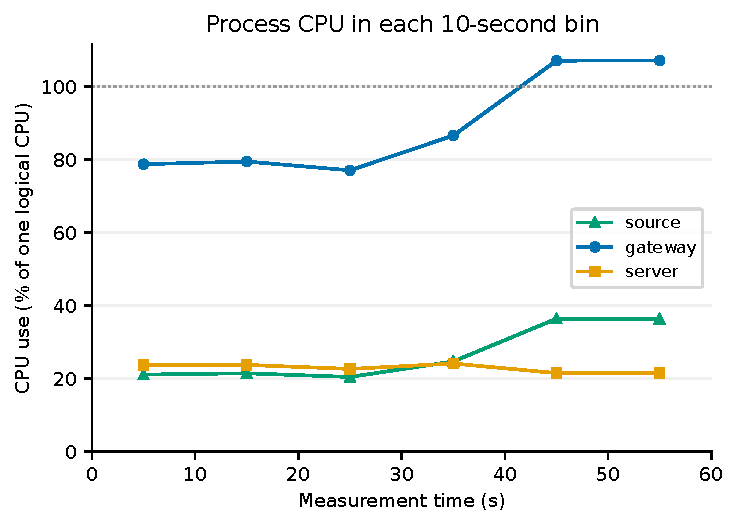
\includegraphics[width=\columnwidth]{figures/appendix_within_run_cpu.pdf}
    \caption{Process CPU consumption in consecutive 10-second bins
    of the 32-equivalent, repeat-1 run. CPU use is normalised to one
    logical CPU. This is one run, with no across-run error bars.}
    \label{fig:e1story-within-cpu}
\end{figure}

Gateway CPU consumption increased from approximately 77--80\% in
the first 30 seconds to approximately 107\% in the final 20 seconds,
despite unchanged configured publishing rates. Source CPU consumption
also increased. The measurements reveal changing execution behaviour
but do not establish its cause.

Queue occupancy was integrated separately within the same 10-second
bins and divided by bin duration. The analysis verifies that
duration-weighted bin averages recover the validated whole-window
CPU and queue statistics.

\begin{figure}[htbp]
    \centering
    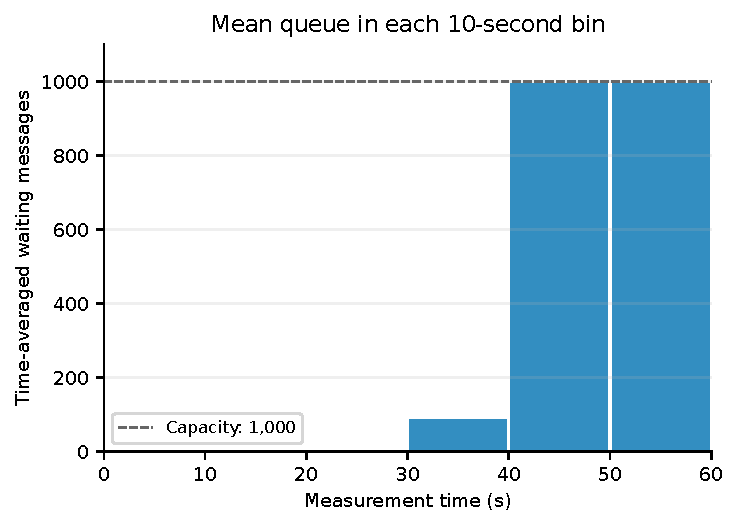
\includegraphics[width=\columnwidth]{figures/appendix_within_run_queue.pdf}
    \caption{Time-averaged FIFO occupancy in the same 10-second bins.
    The dashed line marks the 1,000-message capacity. These are
    within-run time averages rather than averages of three repetitions.}
    \label{fig:e1story-within-queue}
\end{figure}

Mean occupancy was approximately one message in each of the first
three bins, rose to 92.82 in the 30--40 second bin, and reached
approximately 999.6 in the final two bins. Queue growth coincided
with the CPU changes. These observations justify reporting the
variability, but coincidence does not establish a causal mechanism.
